\subsection{Scenario III: Rankine Eddy}
\label{sec:eval:s3}
\begin{figure*}[!t]
\centering
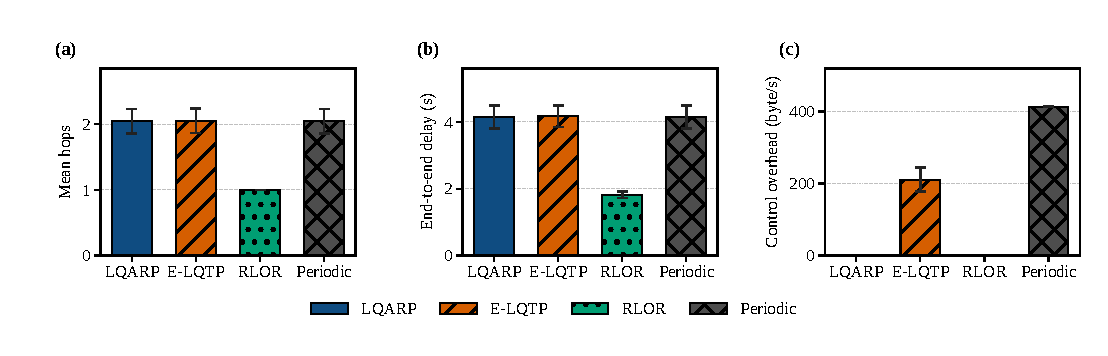
\includegraphics[width=\textwidth]{elqtp_figs/fig5_scenario3_protocols}
\caption{Scenario~III at $V_{\mathrm{eddy}}=2\,\mathrm{m/s}$: hops,
delay, and $O_{\mathrm{ctrl}}$. Error bars are the five-seed sample
standard deviation.}
\label{fig:scenario3_protocols}
\end{figure*}

Table~\ref{tab:s3_protocols} and Fig.~\ref{fig:scenario3_protocols}
repeat the four-protocol comparison under the eddy.
E-LQTP again matches LQARP (PDR $0.9989\pm 0.0018$, hops
$2.050/2.046=1.002\times$, delay $4.167\,\mathrm{s}$ versus
$4.146\,\mathrm{s}$, energy $1.101\times 10^{-2}$ versus
$1.099\times 10^{-2}\,\mathrm{J/bit}$, node-exit packet losses
$0.80\pm 1.30$ for both, VOID $=0$) at
$211\pm 34\,\mathrm{byte/s}$ versus
$413.42\,\mathrm{byte/s}$ ($0.51\times$).
First-fire is $0.708\pm 0.059$; mean exits are $6.40\pm 1.14$ of
$40$, identical across protocols.
The leftover $0.2\%$ hop difference is $N_{\mathrm{stab}}$ with the
trigger on.
A separate five-seed run with $\beta_1=\beta_2=1$ together, outside
the one-at-a-time sweep of Table~\ref{tab:beta_sweep}, produced
$3.250\pm 0.141$ hops against LQARP's $2.046\pm 0.187$
($1.59\times$).
That increase is the scale-mismatched $c_{\mathrm{pred}}$ at an
$O(1)$ weight.
The point is reported only as a diagnostic.

% Scenario III four-protocol headline. Wide 7-col: stay table*.

\begin{table*}[!t]
\caption{Scenario~III at $V_{\mathrm{eddy}}=2\,\mathrm{m/s}$
($N=40$, five seeds, $\beta_1=\beta_2=0$). Entries with $\pm$ are
the sample standard deviation. VOID $=0$.}
\label{tab:s3_protocols}
\centering
\small
\begin{tabular}{lcccccc}
\hline
Protocol & PDR & $T_{\mathrm{e2e}}$ (s) & $E_{\mathrm{bit}}$
  & $O_{\mathrm{ctrl}}$ & Hops & First-fire \\
\hline
LQARP & $0.9989\pm 0.0018$ & $4.146\pm 0.348$ & $1.099\pm 0.098\times 10^{-2}$
  & $0$ & $2.046\pm 0.187$ & --- \\
E-LQTP & $0.9989\pm 0.0018$ & $4.167\pm 0.318$ & $1.101\pm 0.097\times 10^{-2}$
  & $211\pm 34$ & $2.050\pm 0.186$ & $0.708\pm 0.059$ \\
RLOR-insp. & $1.0000\pm 0$ & $1.814\pm 0.093$ & $5.361\times 10^{-3}$
  & $0$ & $1.000\pm 0$ & --- \\
Periodic & $0.9989\pm 0.0018$ & $4.146\pm 0.348$ & $1.099\pm 0.098\times 10^{-2}$
  & $413.42$ & $2.046\pm 0.187$ & $1.000$ \\
\hline
\end{tabular}
\end{table*}


The pair-level trace of Fig.~\ref{fig:trigger_trace} is
Scenario~III pair $(1,2)$.
The three rising edges at $348$, $483$, and $512\,\mathrm{s}$ are
that pair's HELLOs, not the network-wide count.
The network-wide count is $O_{\mathrm{ctrl}}$: the forecast track
is allowed to drift, and a HELLO is charged only on a rising edge
\cite{li2026dse,priel2023consensus}.
